\documentclass[aspectratio=169]{beamer}

\usepackage[utf8]{inputenc}
\usepackage[T1]{fontenc}
\usepackage[brazil]{babel}
\usepackage{amsmath}
\usepackage{graphicx}
\usepackage{tikz}
\usepackage{xcolor}
\usepackage{booktabs}
\usepackage{array}
\usepackage{multicol}
\usepackage{url}

\usetheme{Madrid}

\usepackage{newtxtext}
\usepackage{newtxmath}
\usefonttheme{serif}
\renewcommand{\familydefault}{\rmdefault}

\definecolor{UnBBlue}{RGB}{19,50,105}
\definecolor{UnBGreen}{RGB}{0,110,50}

\newcommand{\logounb}{logoUnB.png}

\addtobeamertemplate{frametitle}{}{%
    \begin{tikzpicture}[remember picture,overlay]
        \node[anchor=north east, xshift=-0.25cm, yshift=-0.15cm]
            at (current page.north east)
            {\IfFileExists{\logounb}{\includegraphics[height=0.65cm]{\logounb}}{}};
    \end{tikzpicture}
}

\setbeamercolor{palette primary}{bg=UnBBlue, fg=white}
\setbeamercolor{palette secondary}{bg=UnBBlue, fg=white}
\setbeamercolor{palette tertiary}{bg=UnBBlue, fg=white}
\setbeamercolor{frametitle}{bg=UnBGreen, fg=white}
\setbeamercolor{title}{fg=white}
\setbeamercolor{structure}{fg=UnBBlue}
\setbeamertemplate{navigation symbols}{}

\graphicspath{{./}}

\newcommand{\techcaption}[1]{\vspace{0.25em}{\scriptsize\emph{Interpretação técnica: #1}}}
\newcommand{\SI}[2]{#1\,#2}

\title[Antenas LoRa/LoRaWAN]{Projeto de Antenas para Sistema de Segurança com LoRa/LoRaWAN}
\subtitle{Botões de segurança no Campus Darcy Ribeiro da UnB}
\author[Carlos Eduardo, Diogo e Jo\~ao Victor]{
  Carlos Eduardo da S. Papa -- 232013390%
  \texorpdfstring{\\[0.2em]}{, }%
  Diogo Godinho Schwartz -- 221006861%
  \texorpdfstring{\\[0.2em]}{, }%
  Jo\~ao Victor Vieira Faria -- 251031598
}
\institute[UnB]{Universidade de Brasília}
\date{Junho de 2026}

\begin{document}

% ============================================================
% SLIDE 1 — CAPA
% ============================================================
\begin{frame}
  \titlepage
\end{frame}

% ============================================================
% SUMÁRIO
% ============================================================
\begin{frame}{Sumário}
\vspace{-0.75em}
\begin{columns}[T,onlytextwidth]
\column{0.48\textwidth}

\textbf{\color{UnBGreen} I — Contexto e Problema}
\scriptsize
\begin{itemize}
  \item Motivação e proposta
  \item Campus Darcy Ribeiro: pontos monitorados
  \item Por que comparar antenas?
\end{itemize}

\vspace{0.5em}
\small\textbf{\color{UnBGreen} II — Fundamentos Técnicos}
\scriptsize
\begin{itemize}
  \item Modelo de enlace e geometria do campus
  \item Parâmetros de antenas e ganho efetivo
\end{itemize}

\vspace{0.5em}
\small\textbf{\color{UnBGreen} III — Antenas Candidatas}
\scriptsize
\begin{itemize}
  \item Antenas omnidirecionais: dipolo, monopolo e comercial
  \item Antenas diretivas: helicoidal, PCB e parabólica
  \item Parabólica: ganho vs.\ abertura de feixe
\end{itemize}

\column{0.48\textwidth}

\small\textbf{\color{UnBGreen} IV — Simulação}
\scriptsize
\begin{itemize}
  \item Módulos LoRa e cenários simulados
  \item Cenário A: FSPL e margens de enlace
  \item Resultados agregados: ranking módulo-antena
\end{itemize}

\vspace{0.5em}
\small\textbf{\color{UnBGreen} V — Análise e Decisão}
\scriptsize
\begin{itemize}
  \item Antenas diretivas: erros e limitações
  \item Discussão: omni vs.\ diretiva
  \item Recomendações finais
\end{itemize}

\vspace{0.5em}
\small\textbf{\color{UnBGreen} VI — Plataforma Web}
\scriptsize
\begin{itemize}
  \item Plataforma de simulação: motivação e Sandbox
  \item Biblioteca de antenas e Link Planner
  \item Topologia do sistema e disponibilização
\end{itemize}

\end{columns}
\end{frame}

% ============================================================
% SLIDE 2 — MOTIVAÇÃO + PROPOSTA (fusão slides 2, 3 e 4)
% ============================================================
\begin{frame}{Motivação e proposta}
\vspace{-1em}
\small
\begin{columns}[T,onlytextwidth]
\column{0.48\textwidth}
\begin{block}{Problema operacional}
\begin{itemize}
  \item Botões de segurança acionam a central via cabeamento externo vulnerável.
  \item Sistema atual sofre com baixa manutenção, falhas de continuidade e exposição mecânica.
  \item Expansão exige obras e custo crescente.
\end{itemize}
\end{block}
\column{0.48\textwidth}
\begin{block}{Proposta: LoRa/LoRaWAN em \SI{915}{MHz}}
\begin{itemize}
  \item Comunicação wireless de longo alcance e baixa taxa.
  \item Topologia em estrela: nós de alarme para gateway central.
  \item Baixo consumo para favorecer recarga solar.
  \item Antenas definem ganho, cobertura e polarização.
\end{itemize}
\end{block}
\end{columns}
\vspace{0.4em}
\begin{block}{Foco do projeto}
Comparar antenas candidatas para nós e gateway com modelo quantitativo baseado na geometria real do campus.
\end{block}
\end{frame}

% ============================================================
\begin{frame}{Campus Darcy Ribeiro: arquitetura e pontos monitorados}
\vspace{-1cm}
\begin{columns}[T,onlytextwidth]
  % Coluna Esquerda: Mapa com legenda
  \column{0.48\textwidth}
  \centering
  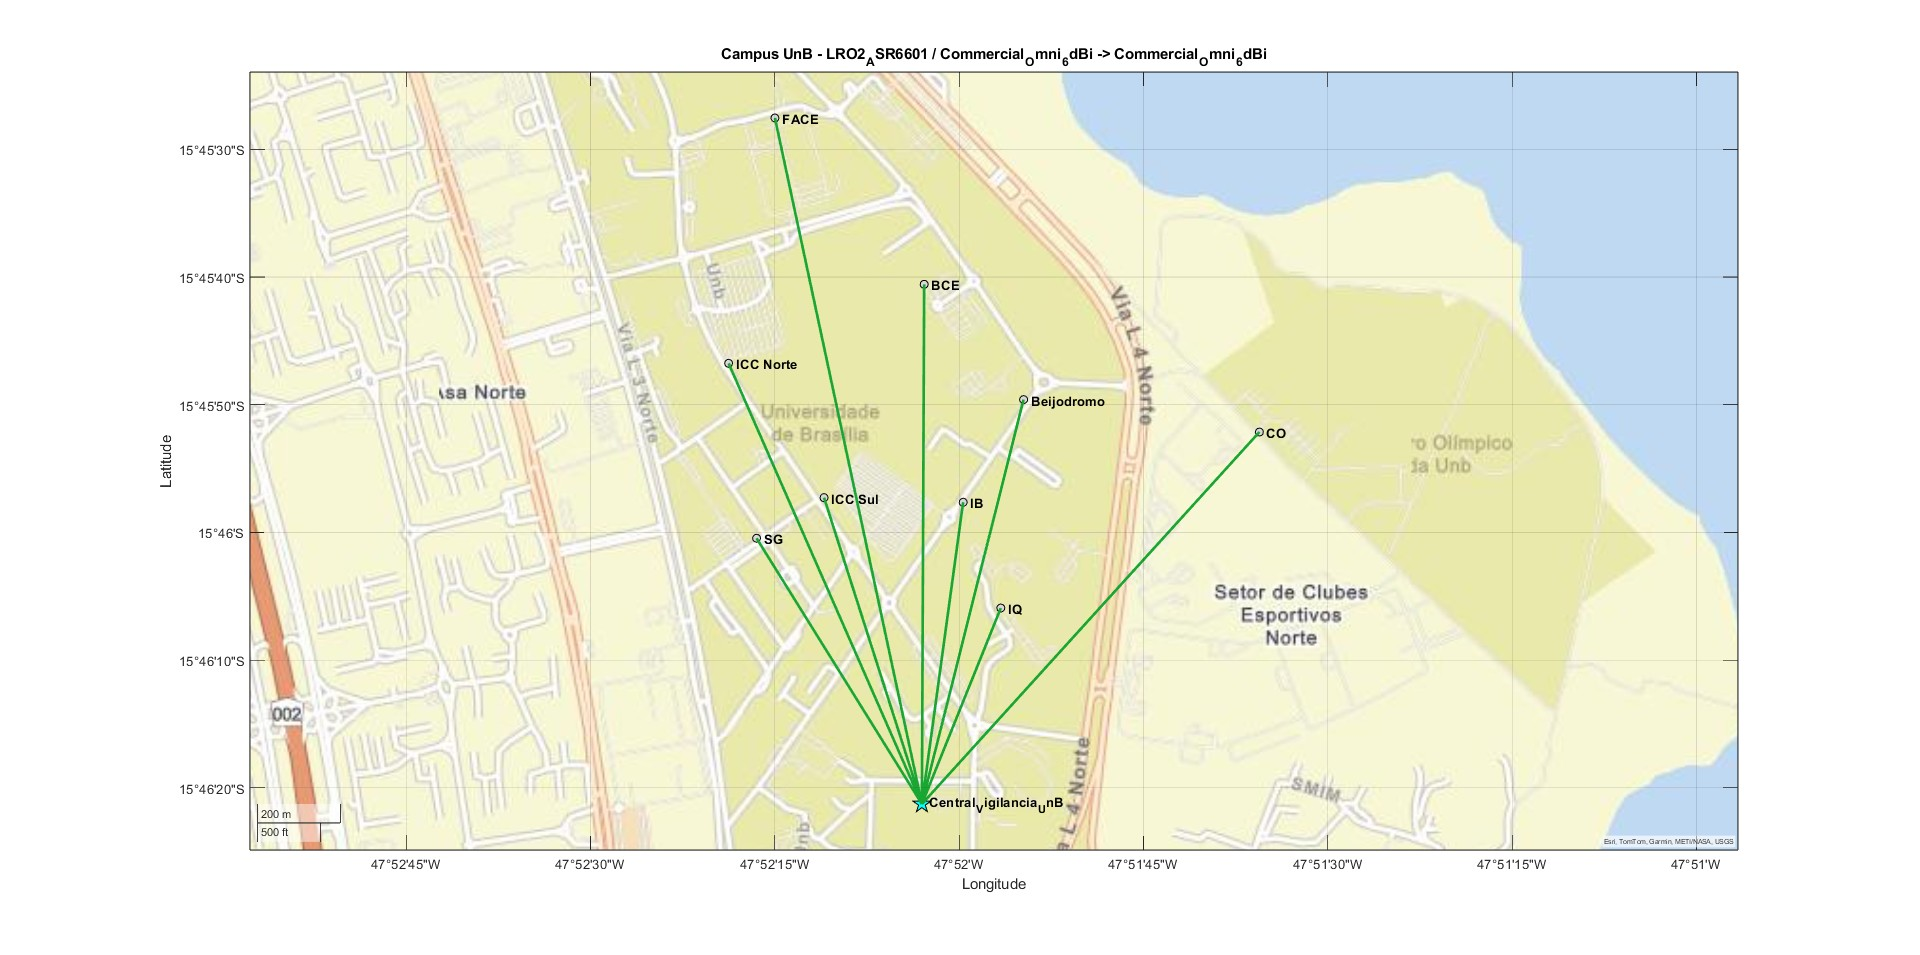
\includegraphics[width=\linewidth,height=0.48\textheight,keepaspectratio]{CampusUnBArranjoMapaSatelite.jpg}\\
  \vspace{0.3em}
  {\scriptsize\color{structure} Fig. 1:} {\scriptsize Distribuição dos 9 pontos de monitoramento no campus.}

  % Coluna Direita: Imagem do poste de vigilância
  \column{0.40\textwidth}
  \centering
  \includegraphics[width=\linewidth,height=0.48\textheight,keepaspectratio]{botaoSeguranca.jpg}\\
  \vspace{0.3em}
  {\scriptsize\color{structure} Fig. 2:} {\scriptsize Estrutura física do poste de vigilância utilizado.}
\end{columns}

\vspace{0.3em}

% Bloco de Geometria na parte inferior
\begin{block}{Geometria e requisitos de cobertura}
  \small
  Os 9 pontos distribuídos geograficamente transmitem para a Central de Vigilância. A variação de azimutes e distâncias de cada enlace dita diretamente a abertura angular necessária para a antena do gateway.
\end{block}

\end{frame}

% ============================================================
% SLIDE 5 — POR QUE COMPARAR ANTENAS (slide 8)
% ============================================================
\begin{frame}{Por que comparar antenas?}
\small
\begin{columns}[T,onlytextwidth]
\column{0.47\textwidth}
\begin{block}{Armadilha comum}
Escolher a antena apenas pelo maior ganho máximo de catálogo ignora a direção do enlace, os nulos do padrão e o papel da antena no sistema.
\end{block}
\begin{block}{Pergunta correta}
Qual antena entrega margem suficiente, instalação viável e cobertura angular adequada para cada função?
\end{block}
\column{0.49\textwidth}
\centering
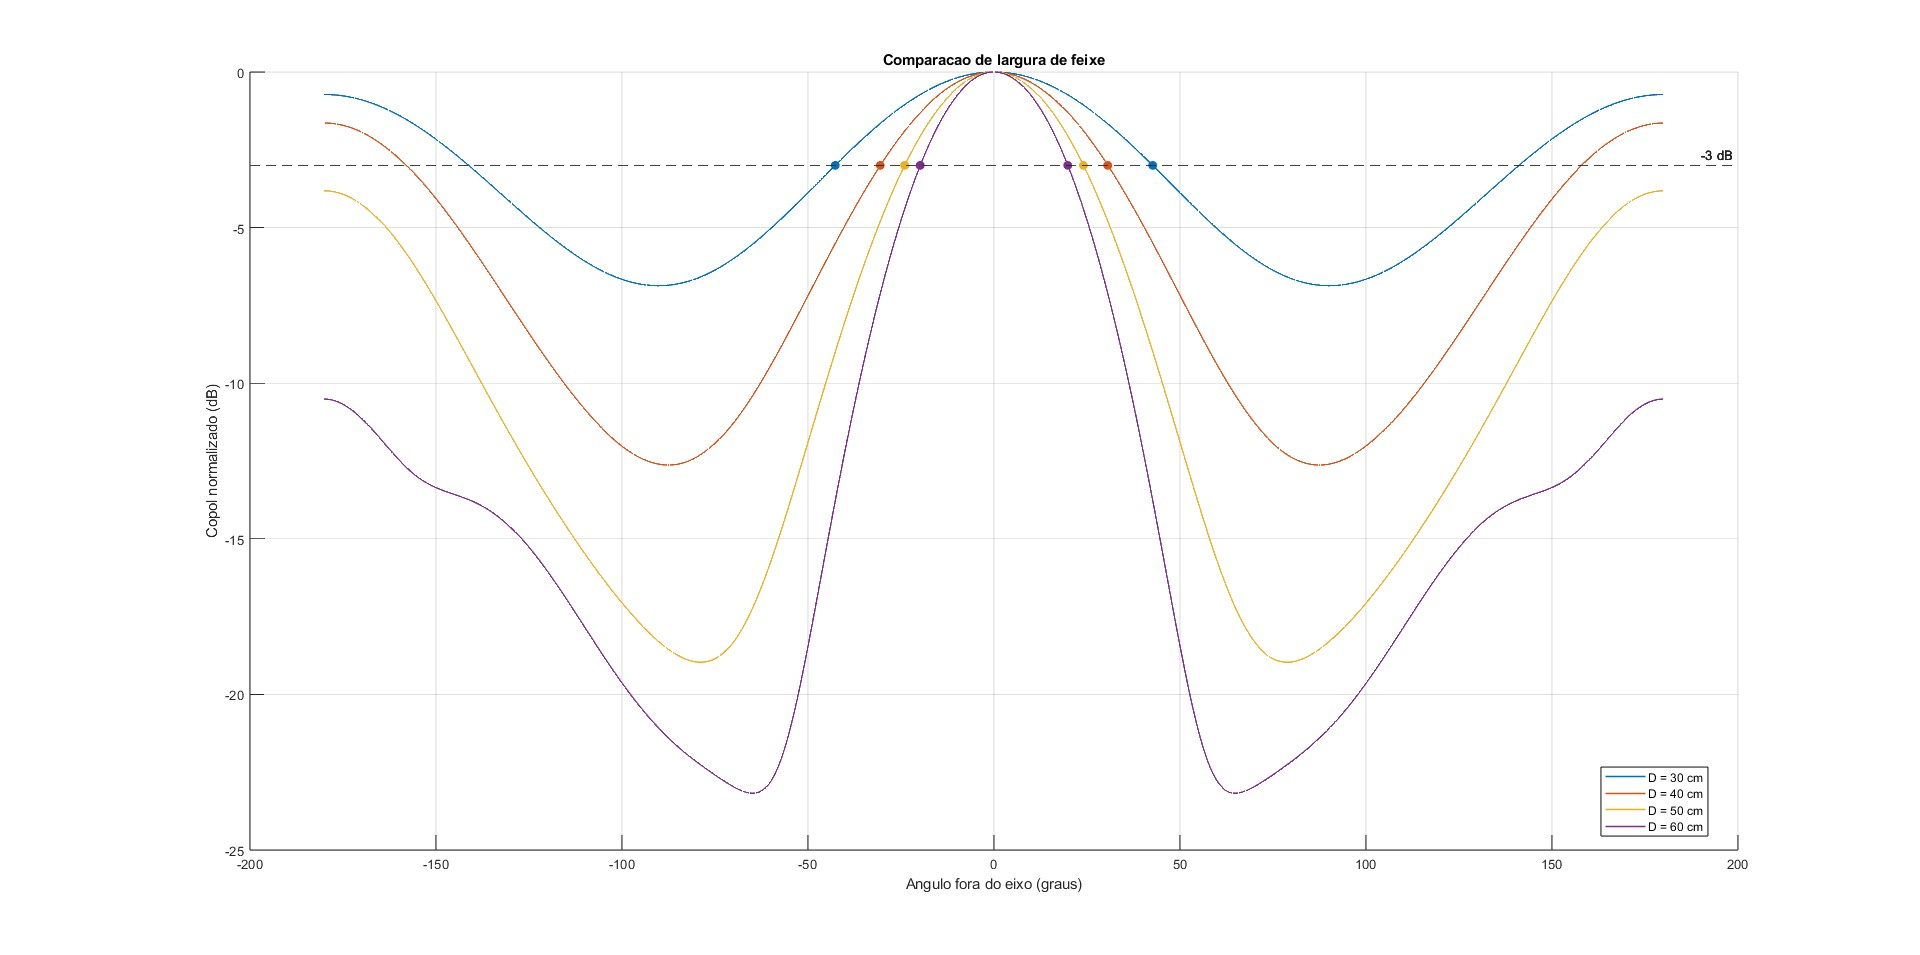
\includegraphics[width=\linewidth,height=0.55\textheight,keepaspectratio]{ComparacaoLarguraDeFeixe.jpg}
\techcaption{O aumento de ganho diretivo geralmente estreita a largura de feixe; o benefício em um enlace apontado pode virar penalidade em recepção multi-azimute.}
\end{columns}
\end{frame}

% ============================================================
% SLIDE 6 — MODELO DE ENLACE + GEOMETRIA (fusão slides 10 e 11)
% ============================================================
\begin{frame}{Modelo de enlace e geometria do campus}
\vspace{-1cm}
\small
\begin{columns}[T,onlytextwidth]

\column{0.48\textwidth}
\begin{block}{Potência recebida}
\[
P_{rx} = P_{tx} + G_{tx} + G_{rx} - FSPL - L_{\mathrm{ad.}}
\]
\end{block}

\begin{block}{Perda em espaço livre}
\[
FSPL = 32{,}44 + 20\log_{10}(f_{\mathrm{MHz}}) + 20\log_{10}(d_{\mathrm{km}})
\]
\end{block}

\begin{block}{Margem}
\[
M_{\mathrm{dB}} = P_{rx,\mathrm{dBm}} - S_{rx,\mathrm{dBm}}
\]
\end{block}

\column{0.48\textwidth}
\begin{block}{Geometria: do mapa ao cálculo}
\begin{itemize}
  \item Coordenadas convertidas para sistema local ENU (Matlab).
  \item Para cada ponto calculou-se: distância 3D, azimute e elevação.
  \item Elevações $< 1{,}1^\circ$, enlaces quase horizontais.
\end{itemize}
\end{block}

\vspace{0.4cm}

\centering
\scriptsize
\begin{tabular}{lrr}
\toprule
Ponto & Azimute p/ GW & Dist. 3D (m) \\
\midrule
FACE & $167.83^\circ$ & 1689.7 \\
BCE  & $180.25^\circ$ & 1251.3 \\
IQ   & $202.05^\circ$ & 509.1 \\
CO   & $222.39^\circ$ & 1212.8 \\
SG   & $147.95^\circ$ & 755.1 \\
\bottomrule
\end{tabular}

\end{columns}
\end{frame}

% ============================================================
% SLIDE 7 — PARÂMETROS DE ANTENA + GANHO EFETIVO (fusão slides 9 e 12)
% ============================================================
\begin{frame}{Parâmetros de antenas e ganho efetivo}
\vspace{-.75cm}
\begin{block}{}
\centering\small
$G_{\mathrm{efetivo}} = G(\theta,\phi)
\qquad\text{ou}\qquad
G_{\mathrm{efetivo}} = G(\alpha_{\mathrm{fora\ do\ eixo}})$
\end{block}
\vspace{0.2em}
\begin{columns}[T,onlytextwidth]
\column{0.52\textwidth}
\scriptsize
\begin{tabular}{p{0.30\linewidth}p{0.64\linewidth}}
\toprule
Parâmetro & Papel no projeto \\
\midrule
Ganho        & Efetivo na direção do enlace — não apenas o máximo de catálogo. \\[2pt]
Diretividade & Cobre múltiplos azimutes ou concentra energia em um boresight. \\[2pt]
Polarização  & Vertical em nós e gateway; descasamento gera perda adicional. \\[2pt]
$S_{11}$     & Casamento de impedância; valores mais negativos reduzem reflexão. \\[2pt]
Largura de feixe & Define tolerância angular e região de cobertura efetiva. \\
\bottomrule
\end{tabular}

\column{0.44\textwidth}
\scriptsize
\begin{itemize}
  \setlength{\itemsep}{4pt}
  \item \textbf{Dipolo/monopolo:} enlaces quase horizontais ficam próximos de $\theta=90^\circ$ (efetivo $\approx$ máximo).
  \item \textbf{Diretivas:} ganho cai quando a direção do enlace se afasta do boresight.
  \item \textbf{Parabólica:} ganho extraído por interpolação das tabelas WebPRAC por ângulo.
\end{itemize}
\end{columns}
\vspace{0.3em}
\begin{block}{Consequência prática}
\small O cálculo usa $G_{tx}$ e $G_{rx}$ efetivos — evita atribuir o ganho máximo para direções onde o padrão tem queda ou nulos.
\end{block}
\end{frame}

% ============================================================
% SLIDE 7 — PARÂMETROS + GANHO EFETIVO (fusão slides 9 e 12)
% ===========================================================
% ============================================================
% SLIDE 8 — ANTENAS OMNI: DIPOLO, MONOPOLO E COMERCIAL (fusão 13, 14 e 17)
% ============================================================
\begin{frame}{Antenas omnidirecionais candidatas (Gateway)}
\small
\begin{columns}[T,onlytextwidth]
\column{0.32\textwidth}
\centering
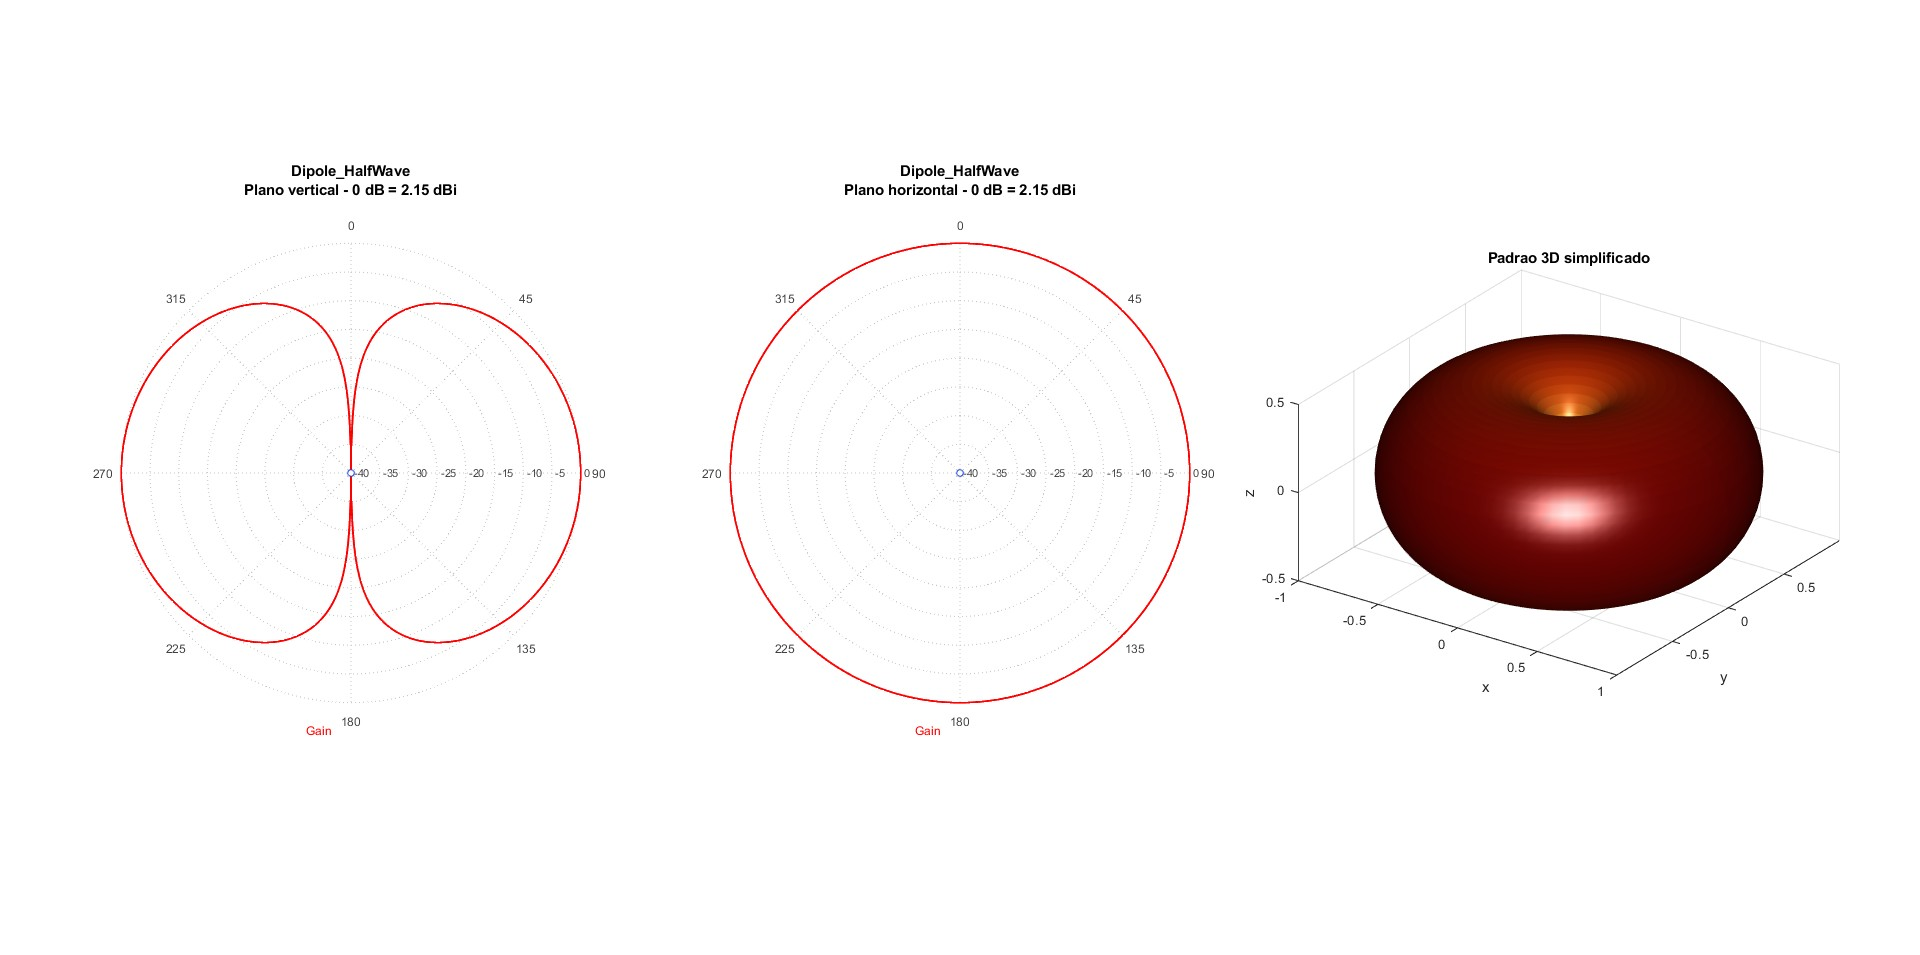
\includegraphics[width=\linewidth,height=0.38\textheight,keepaspectratio]{DipoleHalfWave.jpg}
\textbf{Dipolo $\lambda/2$}\\[0.3em]
\scriptsize
Ganho $\approx$ 2.15 dBi. Referência teórica. Omnidirecional no plano horizontal.

\column{0.32\textwidth}
\centering
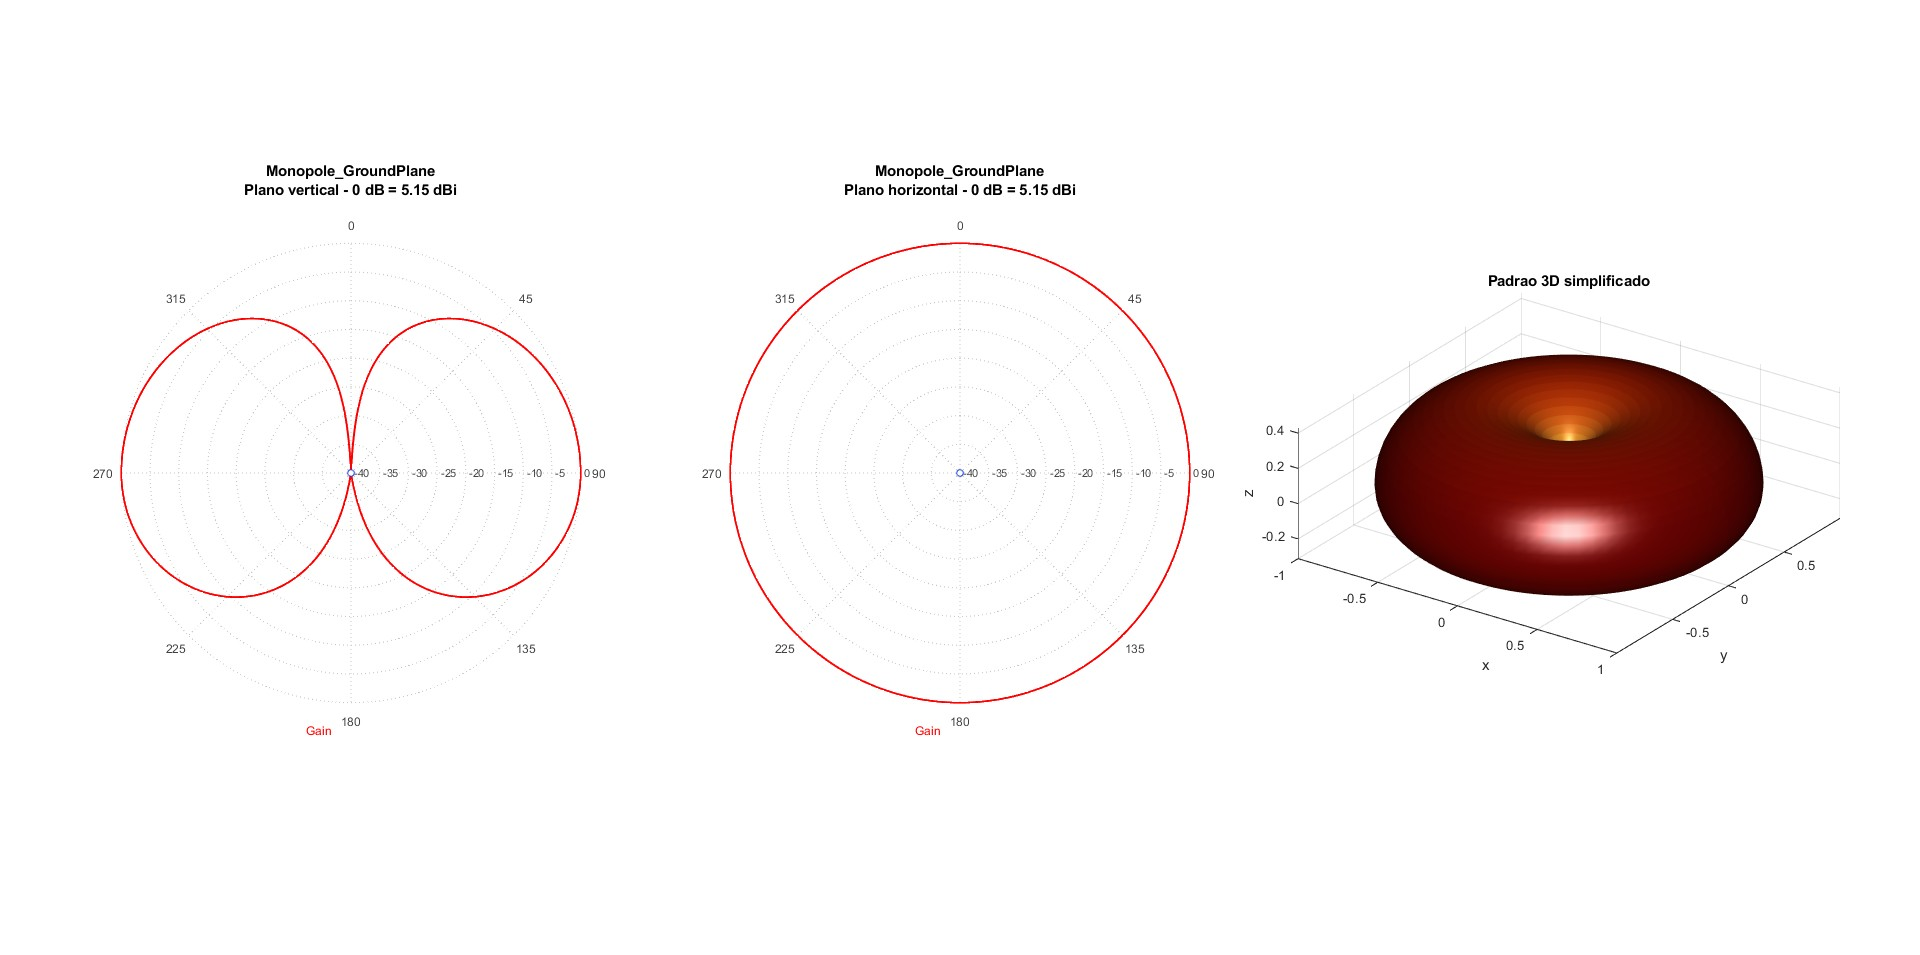
\includegraphics[width=\linewidth,height=0.38\textheight,keepaspectratio]{MonopoleGroundPlane.jpg}
\textbf{Monopolo s/ plano de terra}\\[0.3em]
\scriptsize
Ganho $\approx$ 5.15 dBi. Concentra no horizonte. Forte candidato para nós de alarme.

\column{0.32\textwidth}
\centering
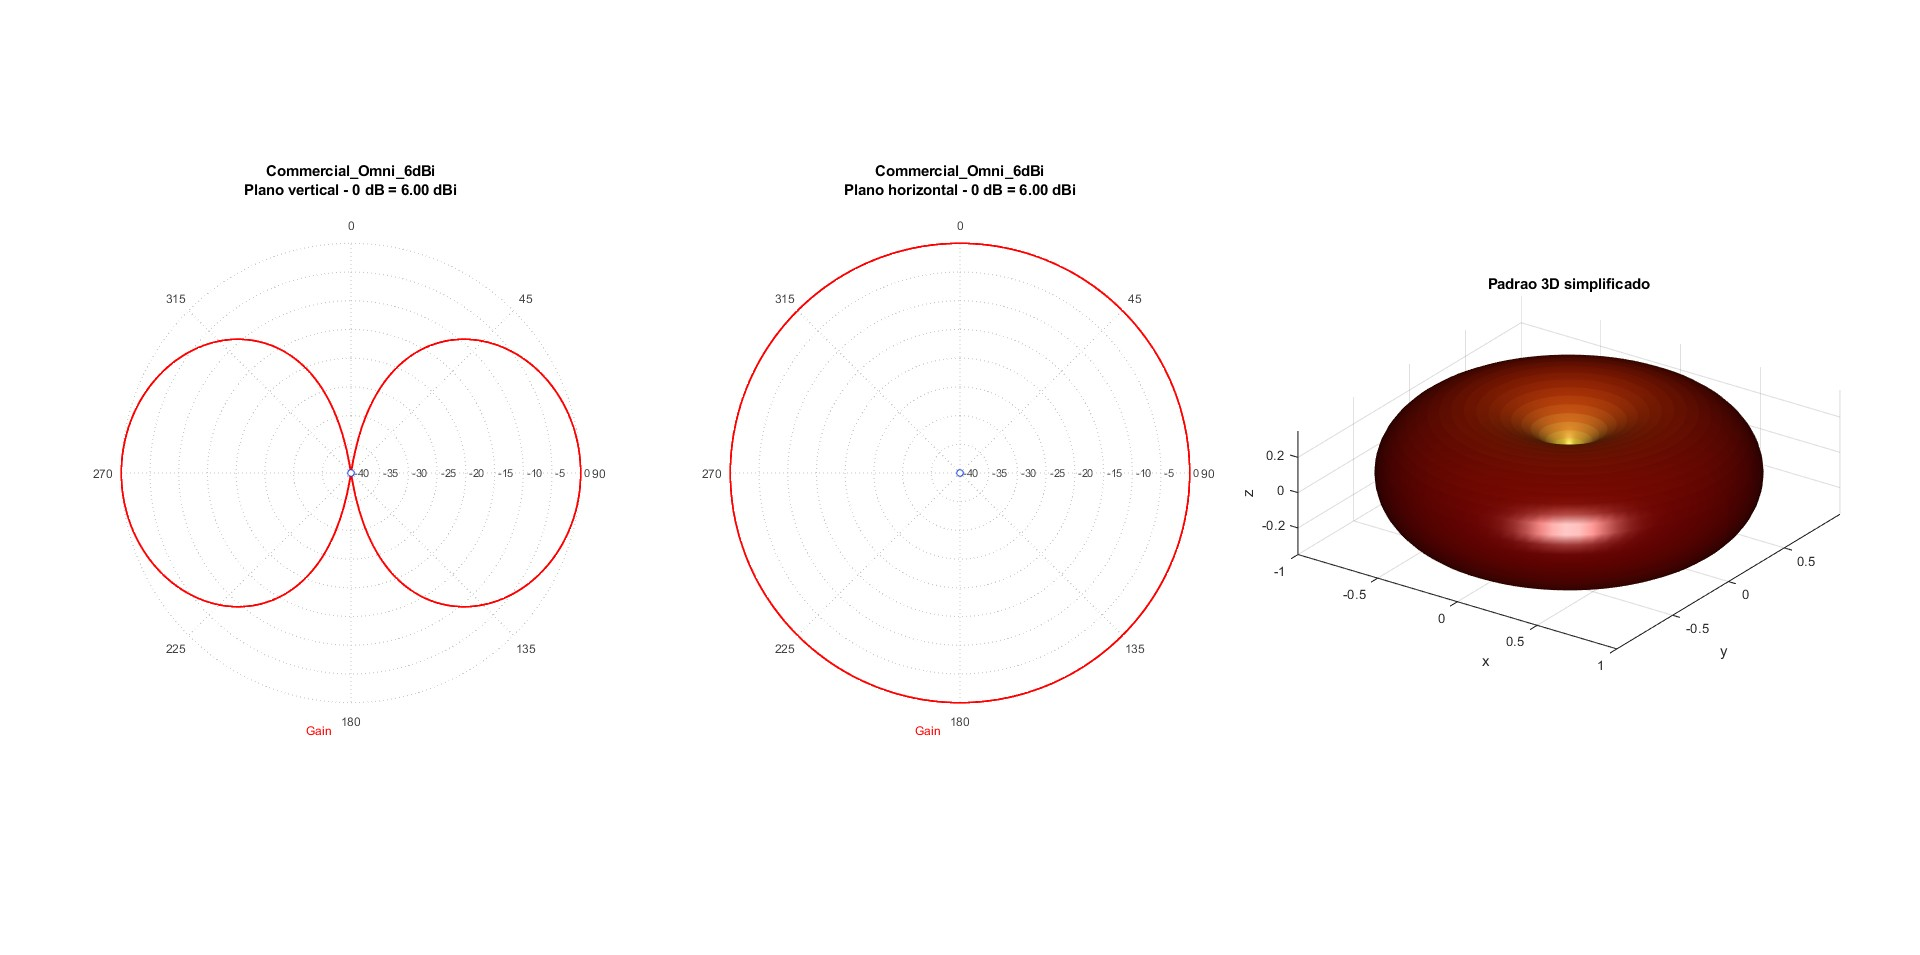
\includegraphics[width=\linewidth,height=0.38\textheight,keepaspectratio]{ComercialOmni6dBi.jpg}
\textbf{Comercial omni 6 dBi}\\[0.3em]
\scriptsize
Ganho 6 dBi nominal. Solução pronta para LoRa. Melhor score agregado na simulação.
\end{columns}
\vspace{0.4em}
\techcaption{Antenas verticais com padrão omnidirecional cobrem todos os azimutes no campus são essencial para o gateway central que recebe de múltiplos pontos.}
\end{frame}

% ============================================================
% SLIDE 9 — ANTENAS DIRETIVAS: HELICOIDAL, PCB E PARABÓLICA (fusão 15, 16 e 18)
% ============================================================
\begin{frame}{Antenas diretivas candidatas (Pontos Remotos)}
\small
\begin{columns}[T,onlytextwidth]
\column{0.32\textwidth}
\centering
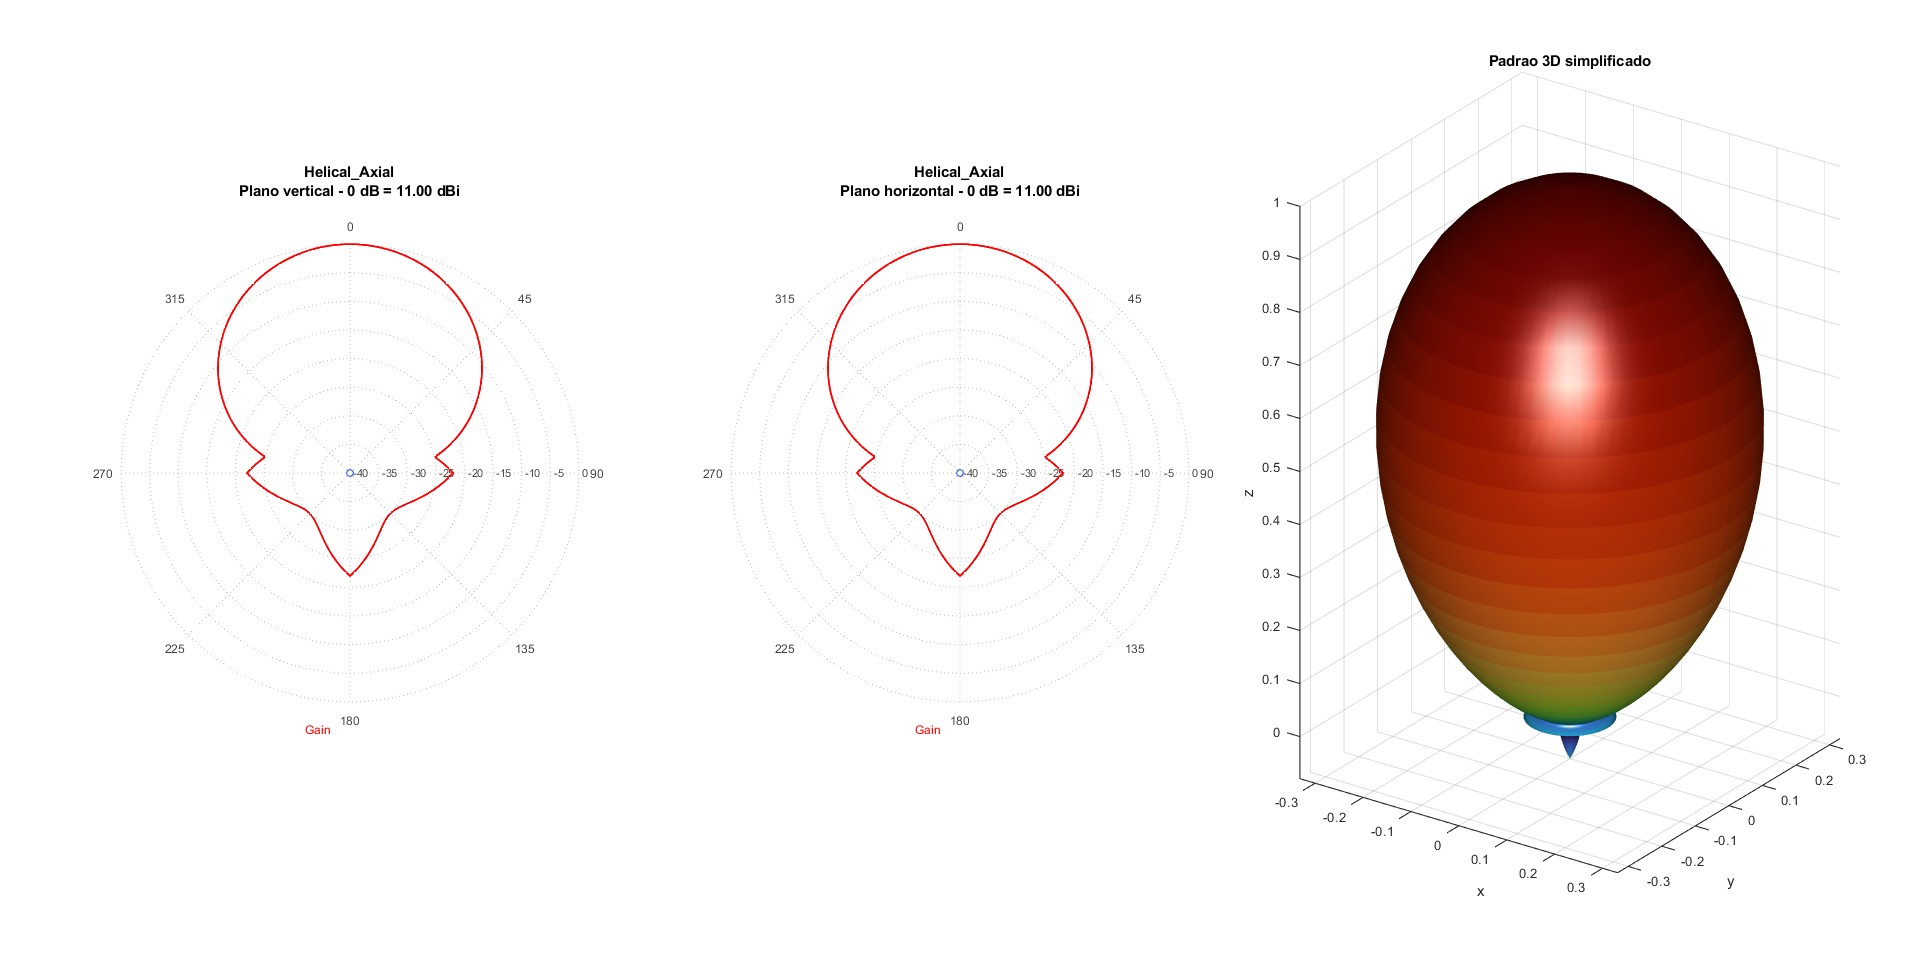
\includegraphics[width=\linewidth,height=0.38\textheight,keepaspectratio]{Helicoidal.jpg}
\textbf{Helicoidal axial}\\[0.3em]
\scriptsize
Alta margem em enlace fixo apontado. Exige orientação mecânica estável. Inadequada como gateway único.

\column{0.32\textwidth}
\centering
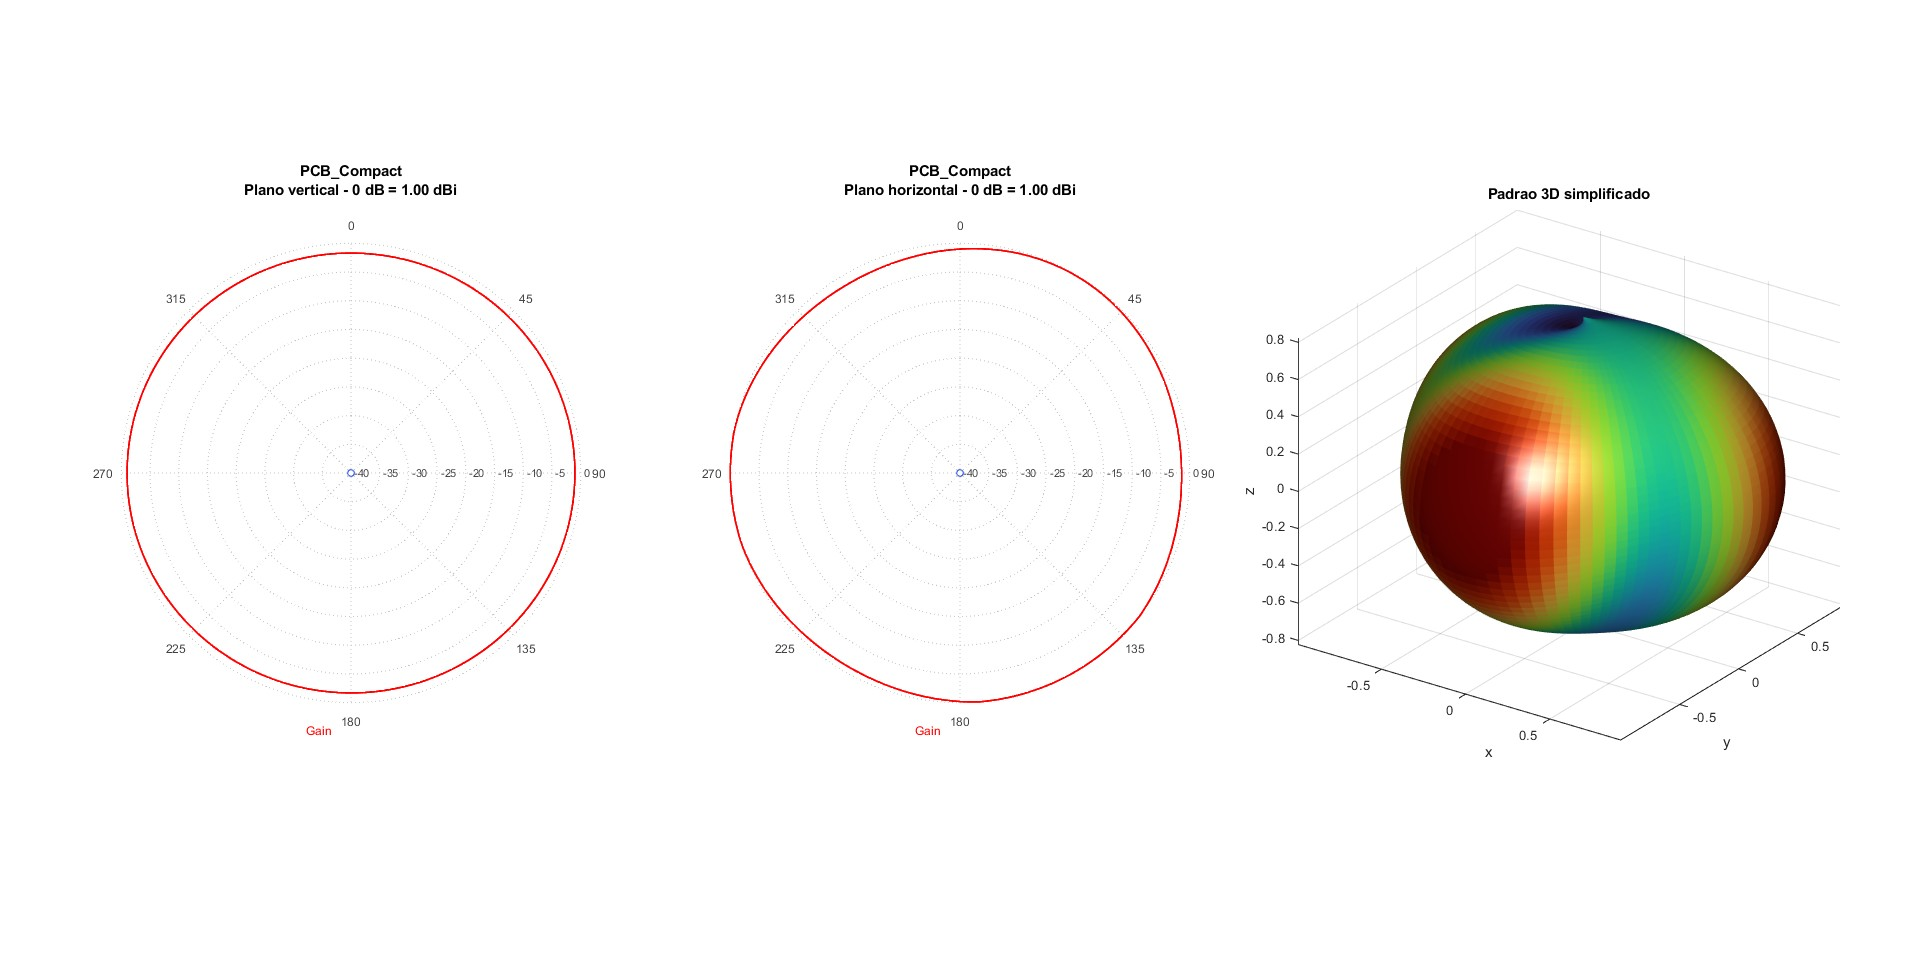
\includegraphics[width=\linewidth,height=0.38\textheight,keepaspectratio]{PCBcompacta.jpg}
\textbf{PCB compacta}\\[0.3em]
\scriptsize
Compacta e barata para nós. Menor ganho e padrão dependente do layout da placa.

\column{0.32\textwidth}
\centering
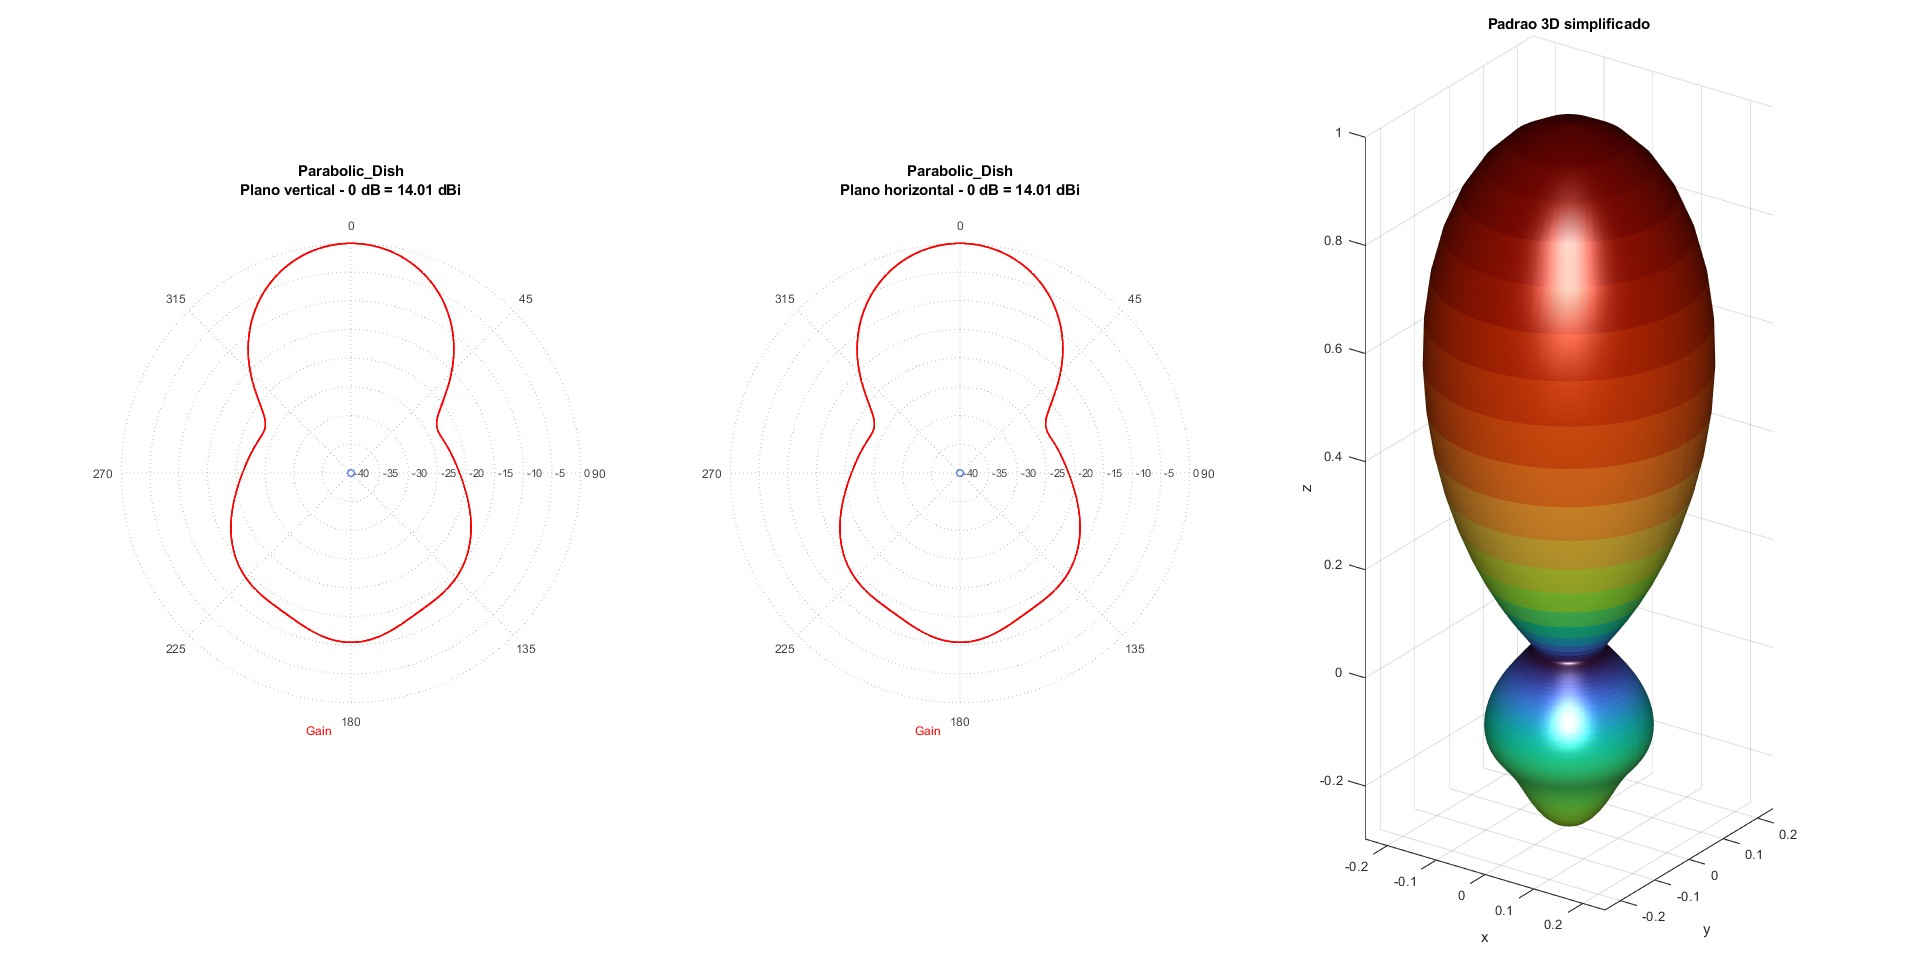
\includegraphics[width=\linewidth,height=0.38\textheight,keepaspectratio]{Parabolica14dBi.jpg}
\textbf{Parabólica ($D \leq 60$\,cm)}\\[0.3em]
\scriptsize
Até 14.01 dBi (PRAC). Maior ganho no boresight, mas cai rapidamente fora do eixo.
\end{columns}
\vspace{0.4em}
\techcaption{Antenas diretivas aumentam margem no boresight, mas exigem apontamento, suporte mecânico e são inadequadas para gateway recebendo de múltiplos azimutes.}
\end{frame}

% ============================================================
% SLIDE 10 — PARABÓLICAS: TABELA D x GANHO + WEBPRAC (fusão 19, 20 e 21)
% ============================================================
\begin{frame}{[Análise] - Parabólica}
\vspace{-0.3em}
\begin{columns}[T,onlytextwidth]
\column{0.54\textwidth}
\scriptsize
\begin{tabular}{rrrrr}
\toprule
$D$ (cm) & $G_{\max}$ PRAC & HPBW PRAC & $G_{\max}$ anal. & HPBW anal. \\
\midrule
30 & 7.99 dBi  & $85.3^\circ$ & 6.96 dBi  & $76.5^\circ$ \\
40 & 10.49 dBi & $61.2^\circ$ & 9.46 dBi  & $57.3^\circ$ \\
50 & 12.42 dBi & $48.0^\circ$ & 11.40 dBi & $45.9^\circ$ \\
60 & 14.01 dBi & $39.7^\circ$ & 12.98 dBi & $38.2^\circ$ \\
\bottomrule
\end{tabular}
\vspace{0.0em}

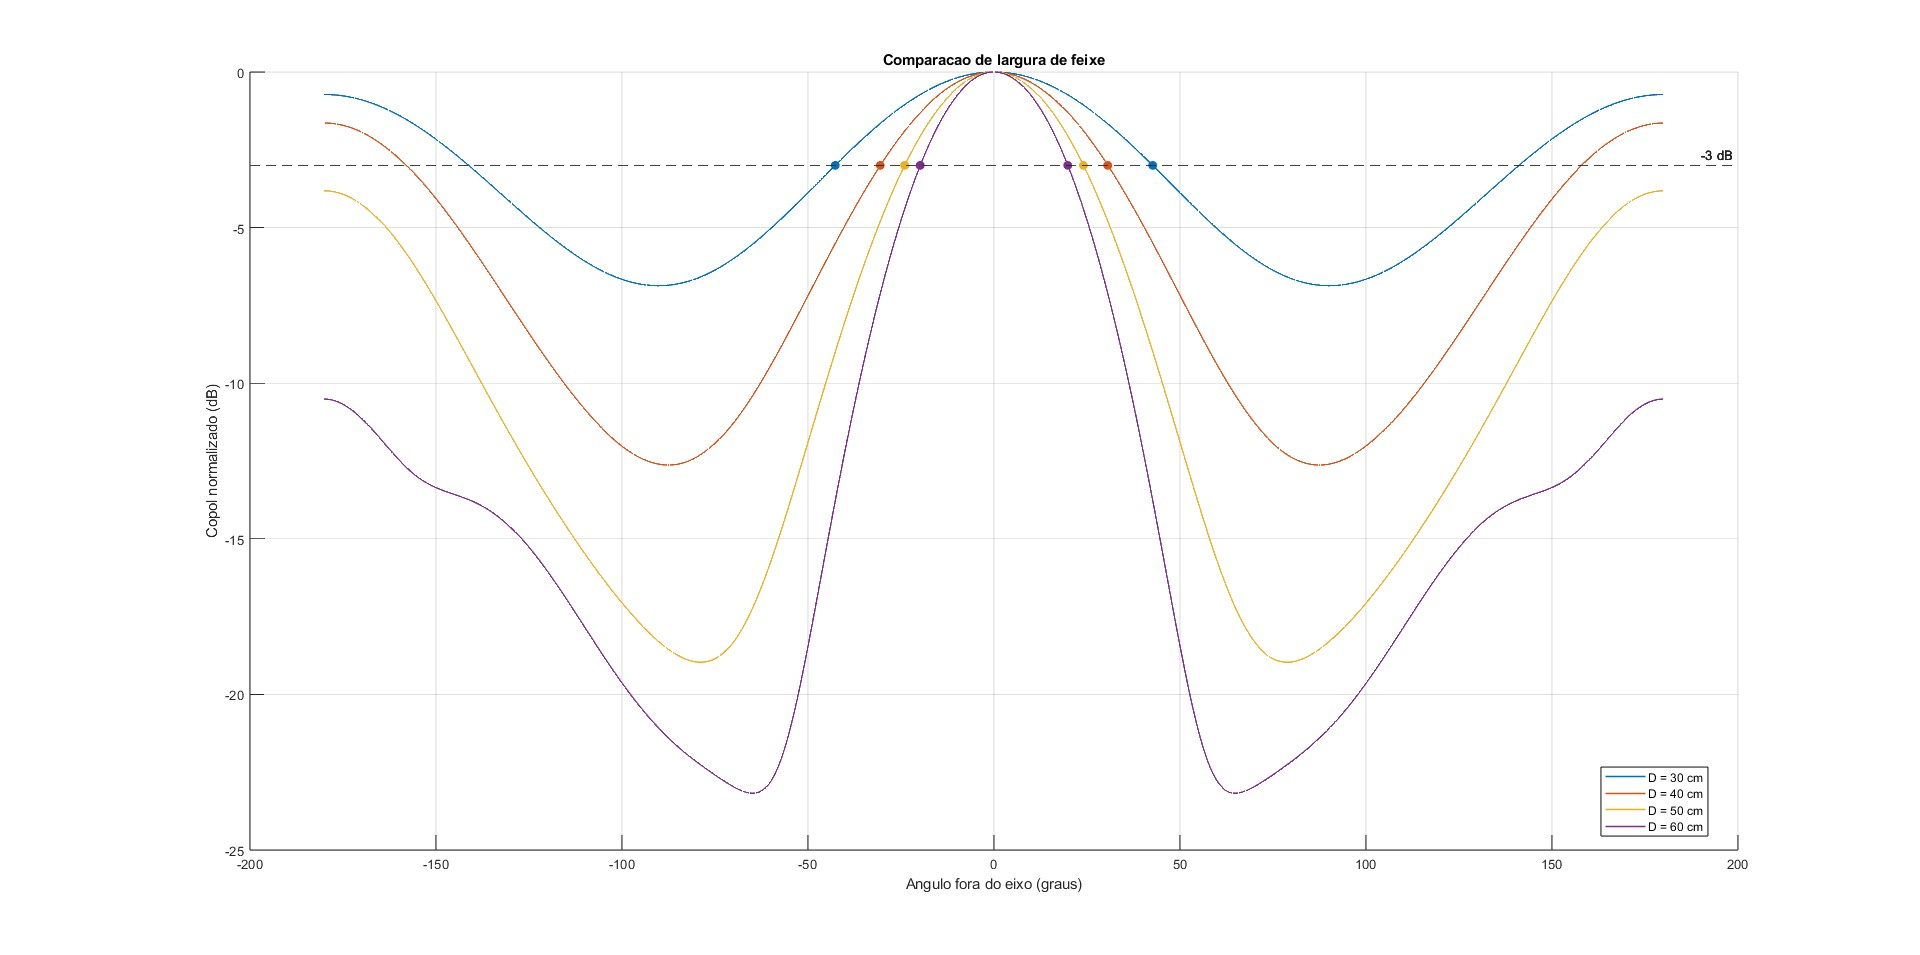
\includegraphics[width=\linewidth,height=0.42\textheight,keepaspectratio]{ComparacaoLarguraDeFeixe.jpg}

\column{0.42\textwidth}
\vspace{-1cm}
\begin{block}{Impacto no campus}
\small
\begin{itemize}
  \item Ganho cresce com $D$, mas HPBW encolhe — margem melhora no eixo, tolerância angular piora.
  \item \textbf{Gateway}: precisa escutar vários azimutes — omni é essencial.
  \item \textbf{Nó fixo}: pode apontar para a central, mas erro de apontamento vira perda de margem.
  \item Mais ganho não implica mais robustez sistêmica.
  \item Limite $D \leq 60$\,cm: viabilidade mecânica.
\end{itemize}
\end{block}
\vspace{0.3em}
\end{columns}
\end{frame}

% ============================================================
% SLIDE 12 — MÓDULOS LORA + CENÁRIOS (fusão slides 23 e 32)
% ============================================================
\begin{frame}{[Validação] Módulos LoRa e cenários de simulação}
\small
\begin{columns}[T,onlytextwidth]
\column{0.52\textwidth}
\scriptsize
\begin{tabular}{p{0.30\linewidth}p{0.18\linewidth}p{0.40\linewidth}}
\toprule
Módulo & $P_{tx}$ máx. & Sensibilidade \\
\midrule
RFM95W 915 MHz & 20 dBm & -139 / -136 / -118 dBm \\
LRO2 ASR6601 & 22 dBm & -138 dBm \\
E220-900T22D & 22 dBm & $\approx -137$ dBm \\
\bottomrule
\end{tabular}
\vspace{0.4em}
\begin{block}{Leitura}
O módulo define potência e sensibilidade. A antena define como essa potência é distribuída no espaço.
\end{block}

\column{0.44\textwidth}
\begin{block}{Cenários simulados}
\scriptsize
\begin{tabular}{p{0.10\linewidth}p{0.80\linewidth}}
\toprule
Cen. & Objetivo \\
\midrule
A & Mesma antena em TX e GW. \\
B & GW omni, TX variando entre antenas. \\
C & TX diretivos apontados, GW omni. \\
D & TX diretivos com erro de apontamento. \\
E & Comparação RFM95W, LRO2, E220. \\
P & Parabólicas 30–60 cm com WebPRAC. \\
\bottomrule
\end{tabular}
\end{block}
\end{columns}
\end{frame}

% ============================================================
% SLIDE 13 — FSPL + PRX (fusão slides 24 e 25, condensada)
% ============================================================

\begin{frame}{[Cenário A] Cálculo de FSPL e margens de enlace}
\vspace{-0.3em}
\begin{block}{\small Cenário de referência: RFM95W, 20 dBm, dipolo em TX e GW, perdas adicionais 19 dB, $S_{rx} = -139$ dBm}
\end{block}
\vspace{0.3em}
\scriptsize
\centering
\begin{tabular}{lrrrrl}
\toprule
Ponto & Dist. 3D (m) & FSPL (dB) & $P_{rx}$ (dBm) & Margem (dB) & Status \\
\midrule
FACE      & 1689.7 & 96.225 & -90.925 & 48.1 & Confortável \\
BCE       & 1251.3 & 93.615 & -88.316 & 50.7 & Confortável \\
Beijódromo & 1004.5 & 91.707 & -86.408 & 52.6 & Confortável \\
IB        &  733.4 & 88.975 & -83.675 & 55.3 & Confortável \\
IQ        &  509.1 & 85.805 & -80.506 & 58.5 & Confortável \\
ICC Sul   &  774.8 & 89.452 & -84.152 & 54.8 & Confortável \\
ICC Norte & 1159.8 & 92.956 & -87.656 & 51.3 & Confortável \\
CO        & 1212.8 & 93.344 & -88.045 & 51.0 & Confortável \\
SG        &  755.1 & 89.228 & -83.931 & 55.1 & Confortável \\
\bottomrule
\end{tabular}
\vspace{0.4em}
\begin{block}{Análise}
\small Mesmo FACE, enlace mais longo com 1689,7 m, apresenta margem de 48,1 dB, muito acima do limiar de 10 dB.
\end{block}
\end{frame}

% ============================================================
% SLIDE 15 — RESULTADOS AGREGADOS (slide 33)
% ============================================================
\begin{frame}{Resultados agregados: combinação módulo-antena}
\small
\scriptsize
\begin{tabular}{p{0.22\linewidth}p{0.24\linewidth}p{0.20\linewidth}rrr}
\toprule
Módulo & Antena TX & Antena GW & Margem mín. (dB) & Média (dB) & Score \\
\midrule
LRO2 ASR6601  & Comercial omni 6 dBi  & Comercial omni 6 dBi & 56.78 & 61.74 & \textbf{98.61} \\
E220-900T22D  & Comercial omni 6 dBi  & Comercial omni 6 dBi & 55.78 & 60.74 & 97.36 \\
LRO2 ASR6601  & Comercial omni 6 dBi  & Monopolo             & 55.93 & 60.89 & 95.95 \\
LRO2 ASR6601  & Helicoidal apontada   & Comercial omni 6 dBi & 58.78 & 63.74 & 94.16 \\
\bottomrule
\end{tabular}
\vspace{0.5em}
\begin{block}{Análise}
A helicoidal apontada tem margem média maior, mas perde praticidade. O ranking agregado favorece a antena comercial omni por combinar margem suficiente, robustez e instalação simples.
\end{block}
\end{frame}
% ============================================================
% SLIDE 17 — DISCUSSÃO DE ENGENHARIA (slide 36)
% ============================================================
\begin{frame}{Discussão: omni vs.\ diretiva}
\small
\scriptsize
\begin{tabular}{p{0.23\linewidth}p{0.35\linewidth}p{0.35\linewidth}}
\toprule
Critério & Favorece omni/monopolo/dipolo & Favorece diretivas \\
\midrule
Cobertura multi-azimute & Gateway central único & Enlace fixo específico \\
Margem máxima & Suficiente em muitos cenários & Maior no boresight \\
Instalação & Simples, leve, repetível & Exige apontamento e suporte \\
Manutenção & Menor sensibilidade a desalinhamento & Maior inspeção mecânica \\
Custo total & Menor integração mecânica & Pode subir com mastro/suporte \\
Flexibilidade & Aceita novos pontos em vários azimutes & Depende de nova orientação \\
\bottomrule
\end{tabular}
\vspace{0.5em}
\begin{block}{Síntese}
\small O projeto não busca a antena de maior ganho absoluto; busca a solução mais coerente com operação, infraestrutura e geometria do campus.
\end{block}
\end{frame}

% ============================================================
% SLIDE 18 — RECOMENDAÇÕES: GATEWAY + NÓS (fusão 37 e 38)
% ============================================================
\begin{frame}{Recomendações finais}
\vspace{-0.3em}
\begin{columns}[T,onlytextwidth]
\column{0.35\textwidth}
\centering
\includegraphics[width=\linewidth,height=0.60\textheight,keepaspectratio]{moduloLora.jpeg}
\small\textbf{Módulo LoRa + antena omni}\\
\scriptsize Antena omni 6 dBi $\sim$915 MHz


\column{0.61\textwidth}
\vspace{0.5em}
\small
\begin{itemize}
  \setlength{\itemsep}{8pt}
  \item \textbf{Gateway:} omni 6 dBi (única opção que cobre todos os azimutes do campus).
  \item \textbf{Nós (poste):} omni 6 dBi ou monopolo (margem confortável e instalação simples).
  \item \textbf{Nós (casos especiais):} PCB compacta para custo; helicoidal ou parabólica apenas em enlace fixo com suporte mecânico adequado.
  \item \textbf{Módulo:} LRO2 ASR6601 (melhor margem agregada da simulação).
\end{itemize}
\end{columns}
\end{frame}
% ============================================================
% SLIDE 19 — PLATAFORMA WEB (fusão 41–46)
% ============================================================
% ============================================================
% SLIDE A — MOTIVAÇÃO + SANDBOX
% ============================================================
\begin{frame}{[Adicional] Plataforma Web de simulação}
\vspace{-0.3em}
\begin{columns}[T,onlytextwidth]
\column{0.54\textwidth}
\centering
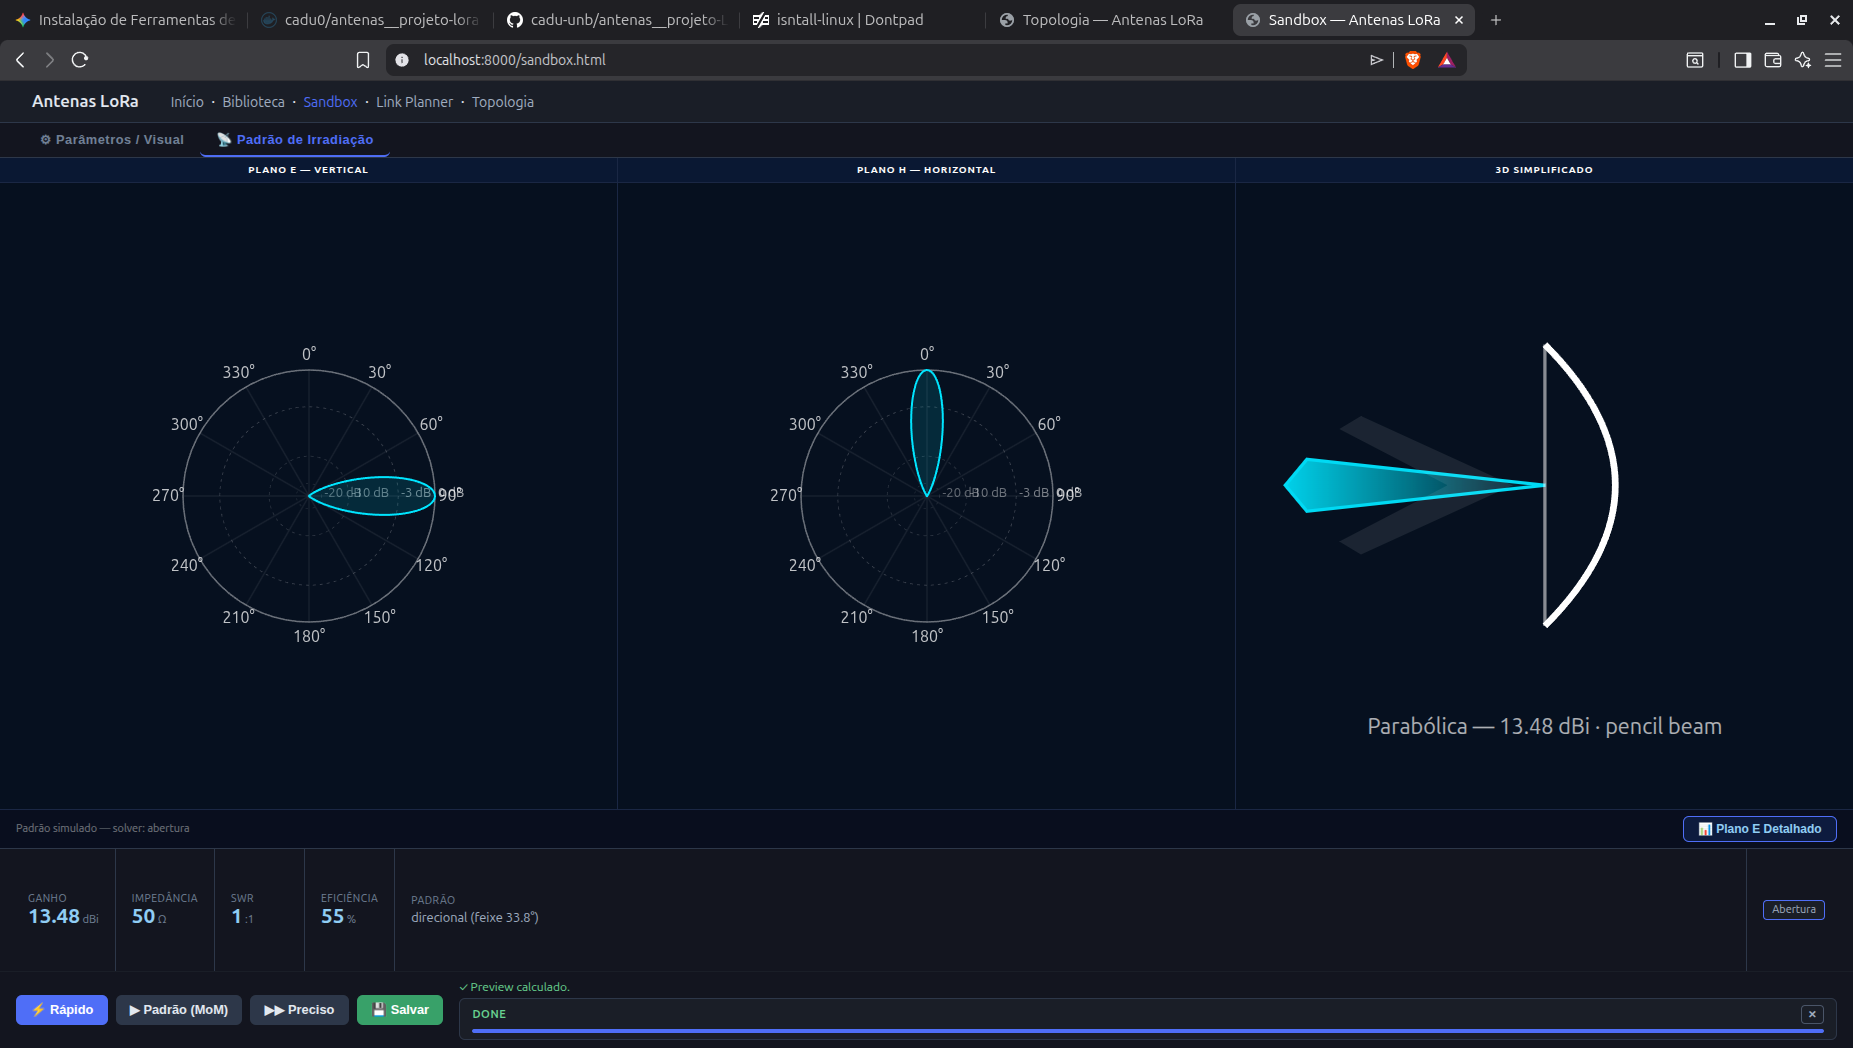
\includegraphics[width=\linewidth,height=0.65\textheight,keepaspectratio]{sandbox-visual.png}
\scriptsize\textit{Sandbox: padrão de radiação e parâmetros configuráveis por tipo de antena.}
\column{0.42\textwidth}
\vspace{-0.5cm}
\begin{block}{Motivação}
\small O WebPRAC calcula ganho por ângulo apenas para parabólicas — não cobre antenas omnidirecionais usadas em LoRa.
\end{block}
\vspace{0.3em}
\begin{block}{Solução}
\small Plataforma própria que estende o WebPRAC para todas as candidatas: dipolo, monopolo, omni, helicoidal, PCB e parabólica.
\end{block}
\vspace{0.3em}
\scriptsize
\textbf{Sandbox:} cria e visualiza antenas por tipo; calcula ganho, impedância, SWR e HPBW com padrão de radiação interativo.
\end{columns}
\end{frame}

% ============================================================
% SLIDE B — BIBLIOTECA + LINK PLANNER
% ============================================================
\begin{frame}{Biblioteca de antenas e Link Planner}
\vspace{-0.3em}
\begin{columns}[T,onlytextwidth]
\column{0.55\textwidth}
\centering
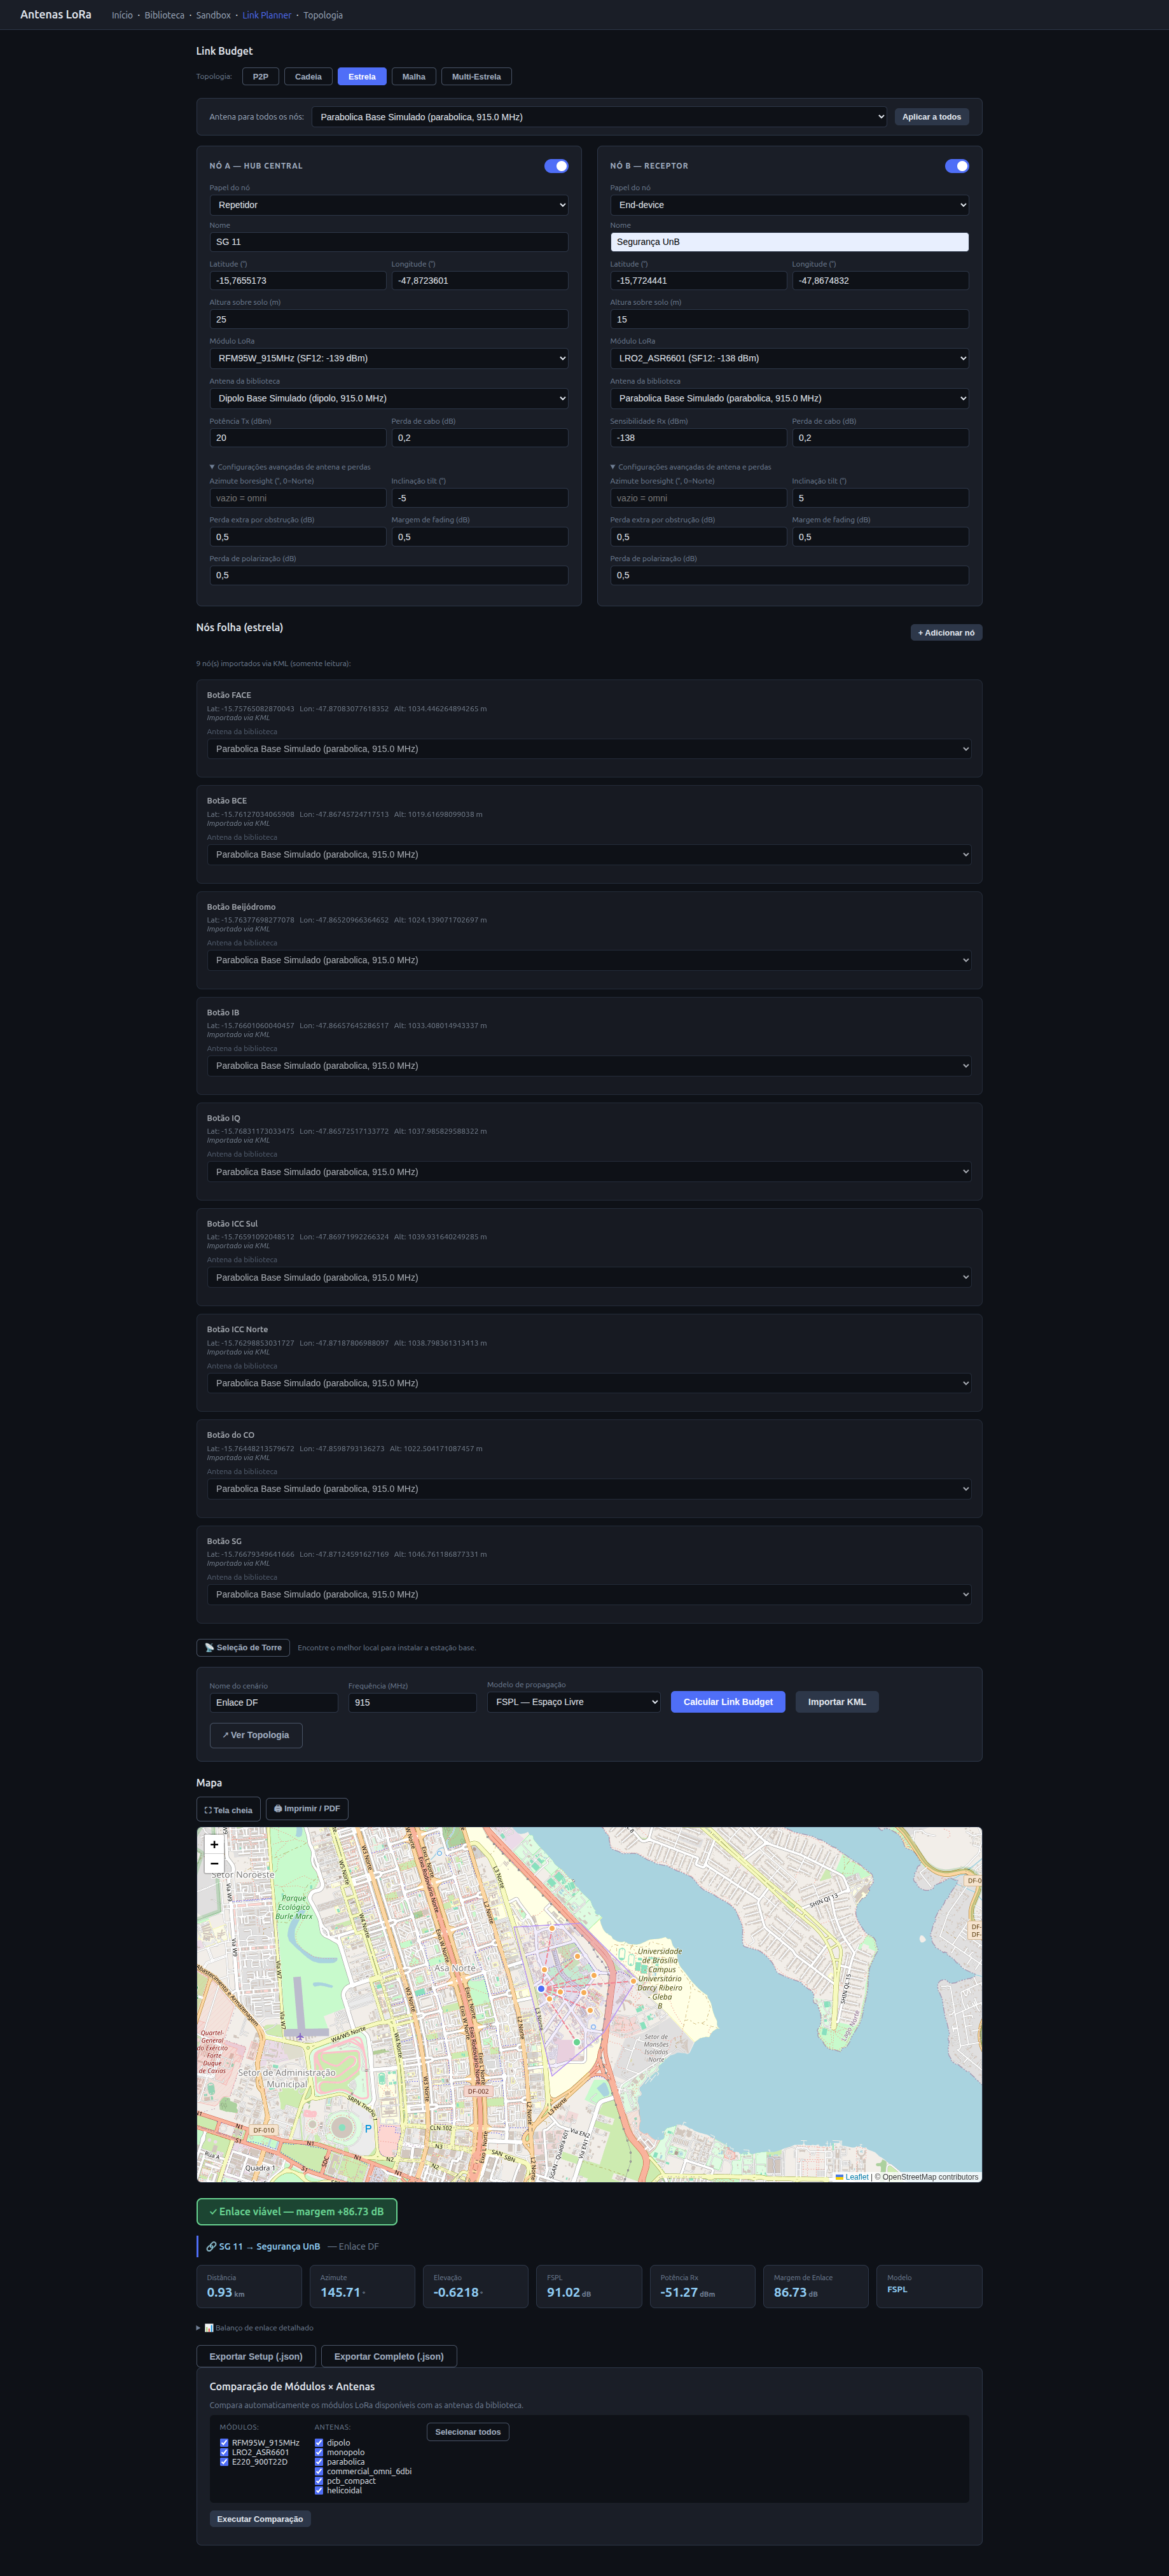
\includegraphics[width=\linewidth,height=0.65\textheight,keepaspectratio]{link-planer.png}
\\
\scriptsize\textit{Link Planner: nós com coordenadas reais, margem por enlace e semáforo de viabilidade.}

\column{0.39\textwidth}
\vspace{-0.5cm}
\begin{block}{Biblioteca}
\scriptsize
\begin{enumerate}
  \item Criar antena no Sandbox.
  \item Salvar com campos físicos: \texttt{gmax\_dbi}, \texttt{hpbw\_deg}, polarização.
  \item Exportar JSON ou reutilizar no Link Planner.
\end{enumerate}
\end{block}
\vspace{0.3em}
\begin{block}{Link Planner}
\scriptsize
\begin{itemize}
  \item Nós com coordenadas reais do campus.
  \item Calcula FSPL, $P_{rx}$ e margem por enlace.
  \item Semáforo: confortável / crítico / falha.
  \item Ganho efetivo direcional por ângulo.
\end{itemize}
\end{block}
\end{columns}
\end{frame}

% ============================================================
% SLIDE C — TOPOLOGIA + DEPLOY
% ============================================================
\begin{frame}{Topologia do sistema e disponibilização}
\vspace{-0.3em}
\begin{columns}[T,onlytextwidth]
\column{0.54\textwidth}
\centering
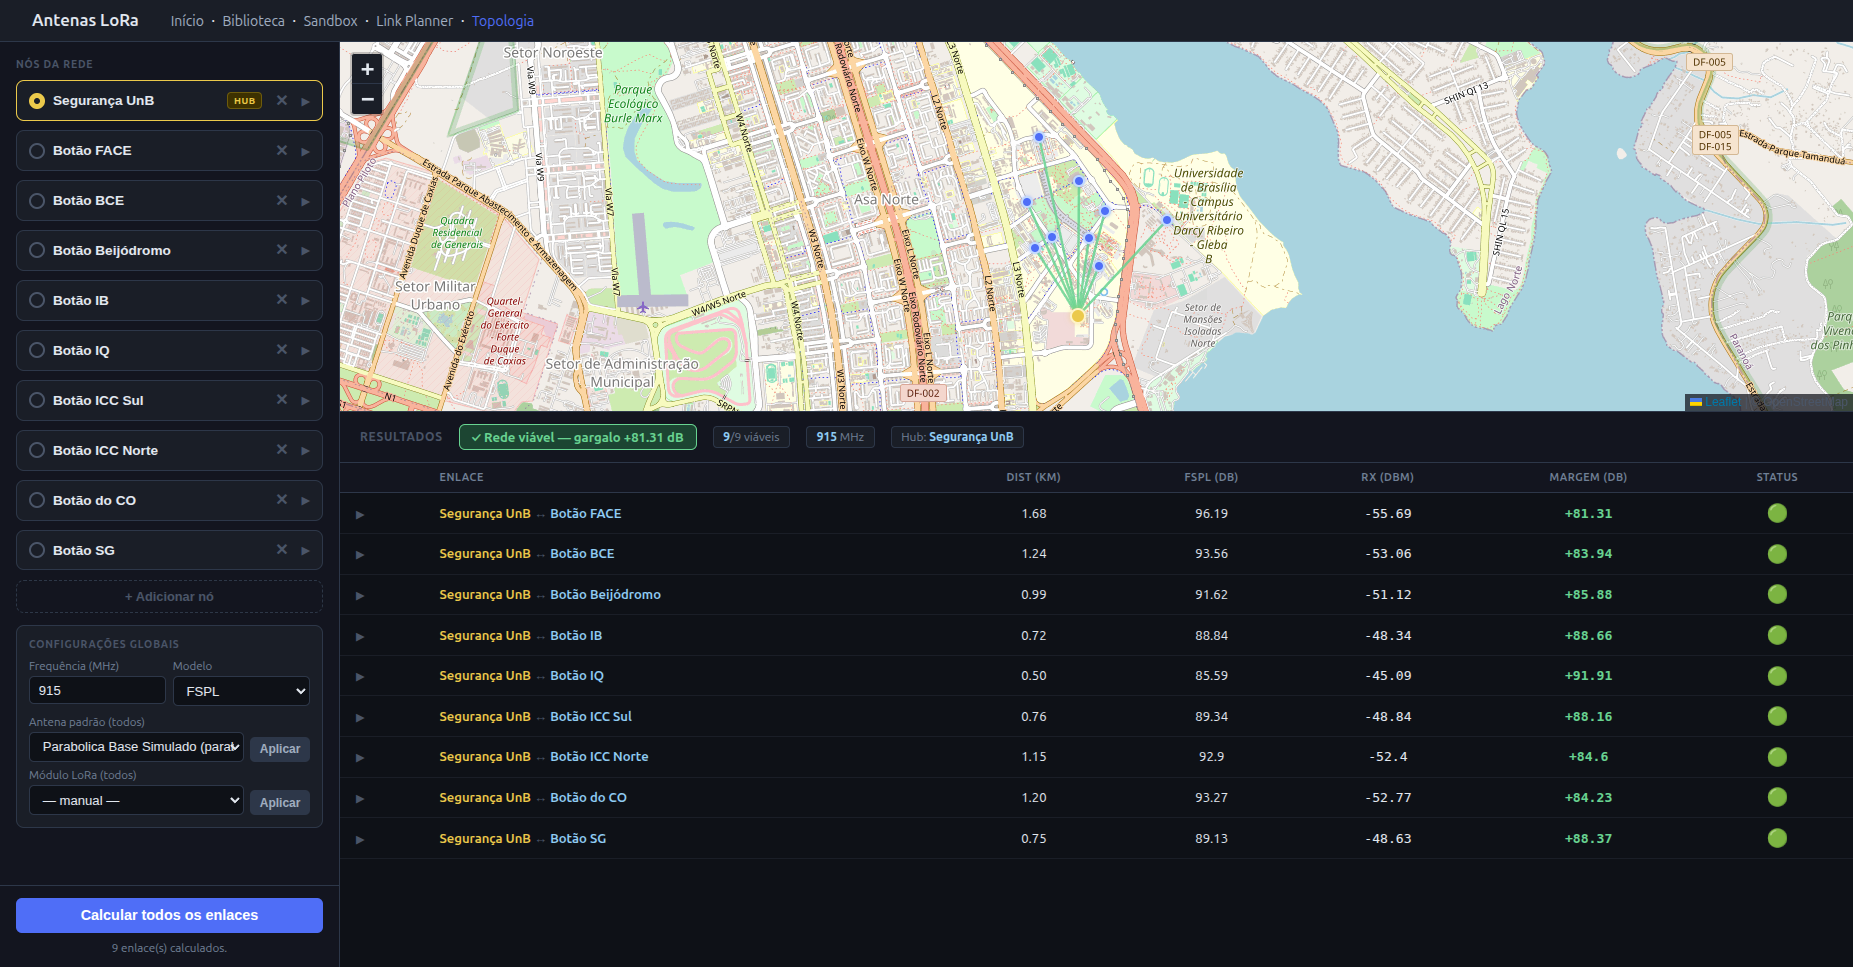
\includegraphics[width=\linewidth,height=0.58\textheight,keepaspectratio]{topologia-segurança.png}
\scriptsize\textit{Topologia em estrela: 9 nós de alarme transmitindo para a Central de Vigilância.}

\column{0.42\textwidth}
\begin{block}{Deploy em um comando}
\scriptsize
\texttt{docker run -p 8000:8000}\\
\texttt{cadu0/antenas\_\_projeto-lora}
\end{block}
\vspace{0.3em}
\begin{block}{Código-fonte público}
\scriptsize
\url{github.com/cadu-unb/antenas__projeto-LoRa}
\begin{itemize}
  \item Backend FastAPI + Pydantic.
  \item Frontend HTML/CSS/JS.
  \item Suite de testes: \texttt{uv run pytest}.
  \item Documentação em \texttt{docs/}.
\end{itemize}
\end{block}
\vspace{0.3em}
\begin{block}{}
\small\centering Pronta para uso educacional e extensão por outros grupos da UnB.
\end{block}
\end{columns}
\end{frame}

% ============================================================
% SLIDE 20 — CONCLUSÃO (slide 47)
% ============================================================
\begin{frame}{Conclusão}
\vspace{-1.5em}
\small
\begin{columns}[T,onlytextwidth]
\column{0.48\textwidth}
\begin{block}{O que o projeto mostrou}
\begin{itemize}
  \item Enlace LoRa é viável para emergências no campus — margens $> 48$\,dB mesmo no ponto mais distante.
  \item A antena comercial omni 6 dBi liderou o ranking agregado: margem suficiente, cobertura em múltiplos azimutes e instalação simples.
  \item Antenas diretivas melhoram margem no boresight, mas perdem robustez para gateway central.
\end{itemize}
\end{block}
\column{0.48\textwidth}
\begin{block}{Contribuições}
\begin{itemize}
  \item Modelagem geométrica com coordenadas reais do Campus Darcy Ribeiro.
  \item Simulação comparativa de 6 antenas e 3 módulos LoRa em múltiplos cenários.
  \item Plataforma Web educacional (Sandbox, Biblioteca, Link Planner), disponível via Docker e GitHub.
\end{itemize}
\end{block}
\end{columns}
\begin{block}{Próximo passo}
Validação de campo: medir RSSI/SNR nos pontos reais e comparar com as margens simuladas.
\end{block}
\end{frame}

% ============================================================
% REFERÊNCIAS (backup, não conta nos 20)
% ============================================================
\begin{frame}{Referências}
\small
\begin{thebibliography}{9}
\bibitem{balanis2005}
BALANIS, Constantine A.
\textit{Antenna Theory: Analysis and Design}.
3.~ed. Hoboken: John Wiley \& Sons, 2005.

\bibitem{lavric2017}
LAVRIC, Alexandru; POPA, Valentin.
Internet of Things and LoRa\texttrademark{} Low-Power Wide-Area Networks: A Survey.
In: \textit{2017 International Symposium on Signals, Circuits and Systems (ISSCS)}.
IEEE, 2017.

\bibitem{terada}
TERADA, Marco Antonio Brasil.
\textit{Material de aula — Antenas e Propagação}.
Universidade de Brasília, Departamento de Engenharia Elétrica.
\end{thebibliography}
\end{frame}

\end{document}